\clearpage
\subsection{premi/client/viewer}
\begin{figure}[h]
\begin{center}
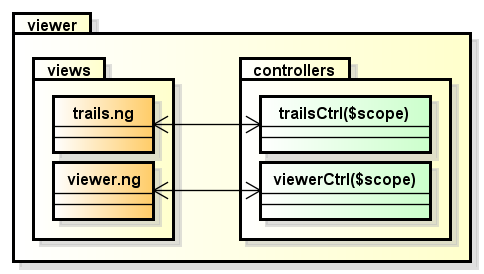
\includegraphics[scale=0.75]{img/diapkg/viewer.png}
\caption{Diagramma del package premi/client/viewer}
\end{center}
\end{figure}


%-------  diagramma di un template %
\subsubsection{premi/client/viewer/views/trails.ng}

\begin{description}
%-------  descrizione del template%
\item[Descrizione] \hfill
	Template della vista associata allo \textit{\$scope} di \textit{trailsCtrl}. Fornisce la lista dei trail associati alla presentazione che l'utente intende visualizzare
\item[Note] \hfill
	\begin{itemize}
			\item per ogni trail fornisce un pulsante per avviare la presentazione
	\end{itemize}
\end{description}

%-------  diagramma di un template %
\subsubsection{premi/client/viewer/views/viewer.ng}

\begin{description}
%-------  descrizione del template%
\item[Descrizione] \hfill
	Template della vista associata allo \textit{\$scope} di \textit{viewerCtrl}. Visualizza la presentazione secondo il trail, o percorso, scelto dall'utente. Sfrutta la libreria esterna impress.js per lo scorrimento dei frame
\item[Note] \hfill
	\begin{itemize}
			\item fornisce i comandi necessari allo scorrimento del trail:
				\begin{itemize}
					\item avanti
					\item indietro
					\item entra in checkpoint
					\item esci da percorso di specializzazione
				\end{itemize}
			\item fornisce un pulsante per tornare indietro al menu dei trail
	\end{itemize}
\end{description}











%-------  diagramma della classe%
\subsubsection{premi/client/viewer/controllers/trailsCtrl}
\begin{figure}[H]
\begin{center}
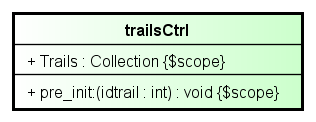
\includegraphics[scale=0.85]{img/diacla/trailsCtrl.png}
\caption{Diagramma della classe premi/client/viewer/controllers/trailsCtrl}
\end{center}
\end{figure}


\begin{description}
%-------  descrizione della classe%
\item[Descrizione] \hfill
	Controller della vista generata dal template \textit{trails.ng}. Fornisce, tramite lo \textit{\$scope}, la lista di tutti i trail creati dall'utente per la presentazione selezionata.
	\\ La dicitura \{\$scope\} nel diagramma UML$_G$ indica che:
\begin{itemize}
\item tutti gli attributi e i metodi pubblici del controller vanno inseriti nello \$scope;
\item tutti gli attributi e i metodi privati del controller appartengono al controller.
\end{itemize}
Vedere la sezione \ref{servizi} per approfondimenti sull'oggetto \$scope.
	

	
%-------  lista degli Attributi%	
\item[Attributi] \hfill
	\begin{description}
		\item[\textbf{- Trails : Collection			}] \hfill
			Collezione di MongoDB dei trail creati dall'utente per la presentazione selezionata. I trail vengono pubblicati prima del caricamento del controller, tramite il pattern publish-subscribe$_G$
	\end{description}
	
	
%-------  lista dei metodi%	
\item[Metodi] \hfill

	% -- inizio metodo -- %
	\begin{description}
		\item[\textbf{\color{blue}+ pre\_init(idtrail)			}] \hfill
			Manda l'utente alla lista dei trail
	\end{description}	

\end{description}



%-------  diagramma della classe%
\subsubsection{premi/client/viewer/controllers/viewerCtrl}
\begin{figure}[H]
\begin{center}
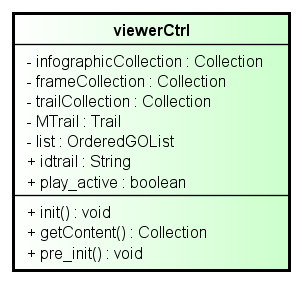
\includegraphics[scale=0.85]{img/diacla/viewerCtrl.png}
\caption{Diagramma della classe premi/client/viewer/controllers/viewerCtrl}
\end{center}
\end{figure}


\begin{description}
%-------  descrizione della classe%
\item[Descrizione] \hfill
	Controller della vista generata dal template \textit{viewer.ng}. Fornisce, tramite lo \textit{\$scope}, gli attributi ed i metodi necessari alla visualizzazione a allo scorrimento della presentazione tramite la libreria impress.js.
	\\ La dicitura \{\$scope\} nel diagramma UML$_G$ indica che:
\begin{itemize}
\item tutti gli attributi e i metodi pubblici del controller vanno inseriti nello \$scope;
\item tutti gli attributi e i metodi privati del controller appartengono al controller.
\end{itemize}
Vedere la sezione \ref{servizi} per approfondimenti sull'oggetto \$scope.
	
	
	
%-------  lista delle classi associate%	
\item[Dipendenze] \hfill
	\begin{itemize}
		\item \textbf{premi/client/presentation/lib/Trail}: per la gestione del percorso della presentazione
		\item \textbf{premi/client/editor/lib/Infographic}: per rappresentare l'infografica come sfondo della presentazione
		\item \textbf{premi/client/presentation/lib/OrderedGOList}: per la gestione della lista degli oggetti grafici dell'infografica
		\item \textbf{premi/client/presentation/lib/signalCtrl}: per la gestione dei signal e degli slot. viewerCtrl usa questa classe per effettuare due chiamate: removeAllSignals() per rimuovere tutti i signal pendenti e initSignal che inizializza i signal per l'oggetto viewer
	\end{itemize}
	
	
%-------  lista degli Attributi%	
\item[Attributi] \hfill
	\begin{description}
		\item[\textbf{- infographicCollection : Collection			}] \hfill
			Contiene l'infografica della presentazione
		\item[\textbf{- frameCollection : Collection			}] \hfill
			Collezione dei frame inseriti all'interno dell'infografica
		\item[\textbf{- trailCollection : Collection			}] \hfill
			Contiene il trail che l'utente intende visualizzare
		\item[\textbf{- MTrail : Trail			}] \hfill
			Oggetto Trail per la gestione del percorso di presentazione
		\item[\textbf{- list : OrderedGOList			}] \hfill
			Oggetto OrderedGOList per il caricamento degli oggetti grafici dei frame e dell'infografica
		\item[\textbf{+ idtrail : String			}] \hfill
			Codice identificativo del trail che l'utente intende visualizzare
		\item[\textbf{+ play\_active : boolean			}] \hfill
			Indica se la riproduzione della presentazione è attiva (\textit{true}) o meno (\textit{false})
	\end{description}
	
	
%-------  lista dei metodi%	
\item[Metodi] \hfill

	% -- inizio metodo -- %
	\begin{description}
		\item[\textbf{\color{blue}+ init() : void			}] \hfill
			Imposta play\_active a \textit{true} e invia un segnale a impress.js per avviare la presentazione
			
	\end{description}
	% -- fine metodo -- %	
	
	% -- inizio metodo -- %
	\begin{description}
		\item[\textbf{\color{blue}+ setSvg() : Collection			}] \hfill
			Per ogni oggetto di tipo shape che appartengono alla presentazione imposta il colore e il path (percorso) di dove si trova l'svg.
			
	\end{description}
	% -- fine metodo -- %	
	
	% -- inizio metodo -- %
	\begin{description}
		\item[\textbf{\color{blue}+ getContent() : Collection			}] \hfill
			Restituisce la lista degli oggetti grafici caricati finora (restituisce \textit{list.getList()})
			
	\end{description}
	% -- fine metodo -- %		
	
	% -- inizio metodo -- %
	\begin{description}
		\item[\textbf{\color{blue}+ pre\_init() : void			}] \hfill
			Prepara gli attributi privati dello \textit{\$scope} per la visualizzazione della presentazione
			
		\begin{description}
			% -- note aggiuntive sul metodo -- %
			\item[Note] \hfill
			\begin{itemize}
					\item preleva l'infografica tramite l'id della presentazione passato come parametro, e la inserisce in infographicCollection
					\item preleva la lista dei frame che sono presenti dentro l'infografica, e li inserisce in frameCOllection
					\item preleva il trail tramite il codice identificativo passato come parametro, e lo inserisce in trailCollection
					\item inserisce i frame e gli oggetti grafici dell'infografica all'interno di list tramite il suo metodo insertGO
					\item imposta lo \textit{\$scope} per reagire agli eventi \textit{nextslide, previousSlide, enterInCheckPoint, returnToCheckPoint} generati dalla vista per lo scorrimento della presentazione
			\end{itemize}
		\end{description}
	\end{description}
	% -- fine metodo -- %		

\end{description}









